\documentclass[12pt]{article}

%%%%%%%%%%%%%%%%%%%%%%%%%%%%%%%%%%%%%%%%%%%%%%%%%%%%%%%%%%%%%
%
% This is the preamble of the .tex file and is the place where you should specify which packages to include and what settings you want for particular commands.
%
%%%%%%%%%%%%%%%%%%%%%%%%%%%%%%%%%%%%%%%%%%%%%%%%%%%%%%%%%%%%%
 
\usepackage{adjustbox, amsmath, amssymb, amsthm, blindtext, bm, bbm, dblfloatfix, esint, fancyhdr, float, graphicx, letltxmacro, marginnote, mathtools, subcaption, xcolor, titlesec, esint}
\usepackage[margin=1.0in]{geometry}
\usepackage{chngcntr}
\usepackage[space]{grffile}
\usepackage[labelfont=bf]{caption}
\usepackage[shortlabels]{enumitem}

% the listings package can be used to include direct code snippets
\usepackage{listings}
\usepackage{color}

\definecolor{codegreen}{rgb}{0,0.6,0}
\definecolor{codegray}{rgb}{0.5,0.5,0.5}
\definecolor{codepurple}{rgb}{0.58,0,0.82}
\definecolor{backcolour}{rgb}{0.95,0.95,0.92}

\lstdefinestyle{mystyle}{
	backgroundcolor=\color{backcolour},   
	commentstyle=\color{codegreen},
	keywordstyle=\color{magenta},
	numberstyle=\tiny\color{codegray},
	stringstyle=\color{codepurple},
	basicstyle=\footnotesize,
	breakatwhitespace=false,         
	breaklines=true,                 
	captionpos=b,                    
	keepspaces=true,                 
	numbers=left,                    
	numbersep=5pt,                  
	showspaces=false,                
	showstringspaces=false,
	showtabs=false,                  
	tabsize=2
}

\lstset{style=mystyle}

\usepackage[colorlinks = true,
            linkcolor = blue,
            urlcolor  = blue,
            citecolor = blue,
            anchorcolor = blue]{hyperref}

% the following lines take care of the headers and footers for each page
\makeatletter
        \newcommand{\rightorleftmark}{%
	\begingroup\protected@edef\x{\rightmark}%
	\ifx\x\@empty
    		\endgroup\nouppercase{\leftmark}
	\else
    		\endgroup\rightmark
  	\fi}
\makeatother

\makeatletter
	\begingroup
  		\catcode`\_=\active
  		\protected\gdef_{\@ifnextchar|\subtextup\sb}
 	\endgroup
	\def\subtextup|#1|{\sb{\textup{#1}}}
	\AtBeginDocument{\catcode`\_=12 \mathcode`\_=32768}
\makeatother

\pagestyle{fancyplain}
\fancyhf{}
\cfoot{ \fancyplain{}{\thepage} }
\renewcommand{\footrulewidth}{0.4pt}

% allow multi-line equations to be split across pages if they occur at the bottom of a page
\allowdisplaybreaks



%%%%%%%%%%%%%%%%%%%%%%%%%%%%%%%%%%%%%%%%%%%%%%%%%%%%%%%%%%%%%
%
% The actual content of the .tex file is enclosed in the \begin{document} and \end{document} tags
%
%%%%%%%%%%%%%%%%%%%%%%%%%%%%%%%%%%%%%%%%%%%%%%%%%%%%%%%%%%%%%
\begin{document}

	\title{Predicting Illegal Substance Use}
	\author{Cynthia Zhang}
	\maketitle

 \begin{center}
     GitHub repository: https://github.com/CynthiaCZ/DATA1030\_project.git
 \end{center}
\section{Introduction}\\
This study aims to produce a classification model that can predict the number of illegal substances used within a year from demographics, personality traits, as well as the frequency of legal substance use. \\
\\
The data is accessed via https://www.kaggle.com/datasets/obeykhadija/drug-consumptions-uci. It was collected in 2015 through an anonymous online survey \cite{fehrman_muhammad_mirkes_egan_gorban_2017}. The Revised NEO five-factor inventory (NEO-FFI-R) was employed to assess traits of neuroticism (N), extraversion (E), openness to experience (O), agreeableness (A), and conscientiousness (C). In addition to that, two additional scales were included to gauge impulsiveness (impulsive) and sensation-seeking (SS). Respondents were asked to provide demographic information including age, gender, level of education, country, and ethnicity, and then to complete the personality evaluation questionnaire. The test subjects were also questioned about their drug consumption history within a list of 19 legal and illegal substances. For each one of the said substances, there are 7 ordinal categories indicating the frequency of substance use. In total, there are 1885 unique study subjects and 32 attributes with no missing values.\\
\\
Most existing studies using this dataset focus on only one or a few drug categories at a time. Usually, the goal is to find predictive trends between personality traits and those specific substances. For example, a study by Qiao et al. concludes that Light Gradient Boosting Machine (LightGBM) model performs well in predicting potential users and usage time of two illegal drugs, Amyl and Meth \cite{qiao_chai_zhang_zhou_chu_2019}. Another study by Adinugroho et al. shows that Extreme Learning Machine (ELM), a type of artificial neural network, has varying accuracy, ranging from 37\% to 86\% in the prediction of the usage duration of each specific substance, legal or illegal \cite{adinugroho_sari_hidayat_2019}. \\
\\
However, this study proposes a more generalized model, focusing on the number of illegal drugs used within a timeframe, making the model potentially useful for psychologists to identify patients prone to drug abuse of any kind. Due to the sensitive nature of illegal drug use, many patients are less willing to disclose such information. Legal substances such as nicotine and alcohol, on the contrary, are less stigmatized and more openly discussed. That is why in this study, five of the legal substances are included as features and are used to predict illegal substance abuse.

\section{Exploratory Data Analysis (EDA)}
The target variable, i.e. the number of illegal substances used within a year is right-skewed (Fig. 1). It ranges from 0 to 7, with a mean of 0.79 and a median of 0.\\
\begin{figure}[!h]
\centering
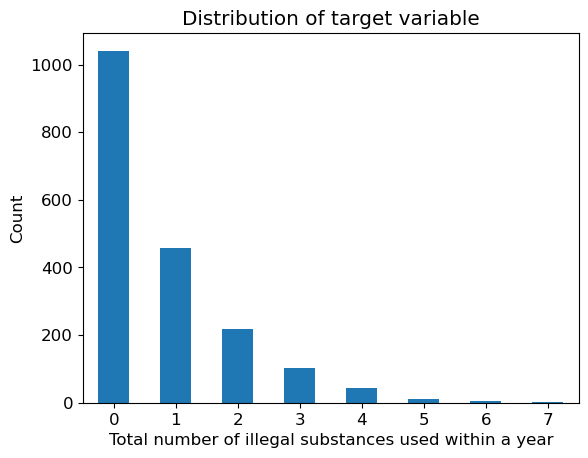
\includegraphics[width=0.75\linewidth]{target_var_barplot.png}
\caption{Bar plot showing the target variable is right-skewed}
\end{figure}
\\
The majority (more than 50\%) of the respondents are from the UK, and more than 25\% are from the US (Fig. 2). The remaining study subjects are from Canada, Australia, the Republic of Ireland, New Zealand, as well as a diversity of other countries. Due to this imbalance, the country feature was excluded from the original study \cite{fehrman_muhammad_mirkes_egan_gorban_2017}, and this study did the same correspondingly.\\
\begin{figure}[!h]
\centering
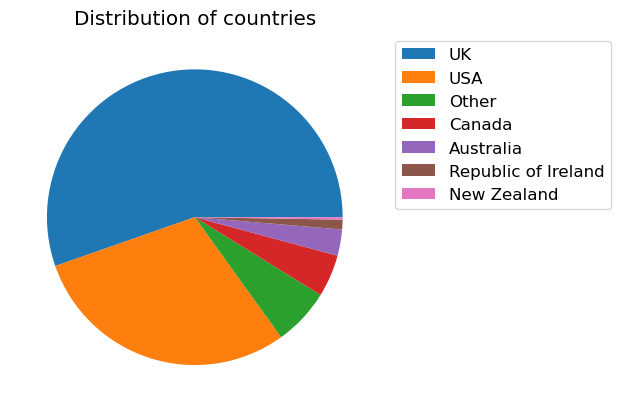
\includegraphics[width=0.75\linewidth]{country_pie.png}
\caption{Pie plot showing most of the respondents are from either the UK or the US}
\end{figure}
\\
According to the linear correlation indicated by the f-statistic, one feature that is strongly correlated to the number of illegal drugs used within a year is the weekly use of nicotine. The left column of the violin plot (Fig. 3) has a wider base, indicating that most non-smokers use zero illegal drugs within the year, whereas the right column shows that smokers tend to use one or more illegal drugs.\\
\begin{figure}[!h]
\centering
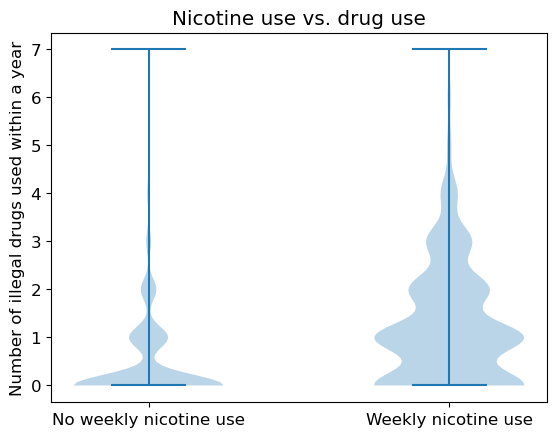
\includegraphics[width=0.7\linewidth]{violinplot_nicotine.png}
\caption{Violin plot showing smokers are more likely to use illegal drugs than non-smokers}
\end{figure}
\pagebreak
\\
Another feature with a strong correlation to drug use is age. As shown in the normalized stacked bar plot (Fig. 4), most people in the youngest age group (18-24) have tried one or more illegal drugs within the year, while people in older age groups tend to use zero or very few illegal drugs. \\
\begin{figure}[!h]
\centering
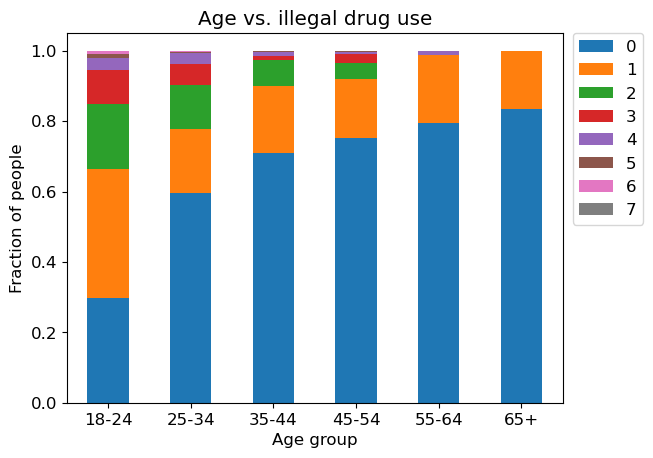
\includegraphics[width=0.7\linewidth]{age_stacked.png}
\caption{Stacked bar plot showing younger people are more likely to use illegal drugs than older people}
\end{figure}
\pagebreak
\\
Among the seven personality traits, the one with the highest f-score is Sensation Seeking (SS). This is illustrated by the heatmap (Fig. 5). People with negative SS scores tend to fewer illegal drugs. As the SS score increases, the number of drugs used within the year increases accordingly, forming the triangular shape at the lower left corner of the heatmap. 
\begin{figure}[!h]
\centering
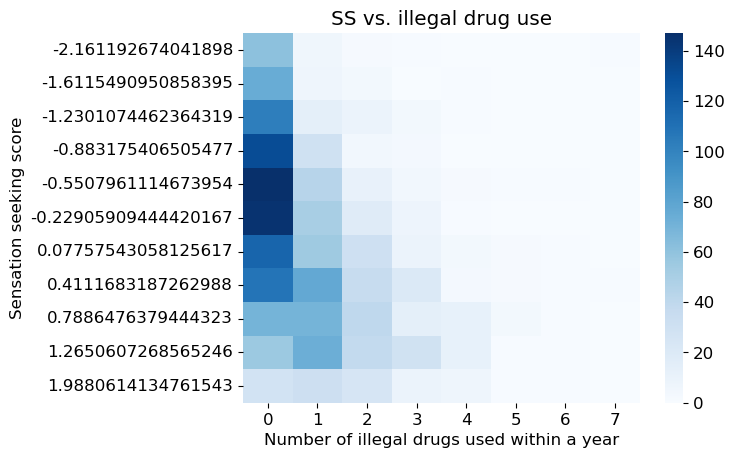
\includegraphics[width=0.7\linewidth]{heatmap_SS.png}
\caption{Heatmap showing Sensation Seeking score is positively correlated to drug use}
\end{figure}
	
\section{Methods}

\subsection{Featuring Engineering}
The original dataset is manipulated using sklearn in the following ways to suit the purpose of this study. First, the ID column and the Semeron column are removed. Semeron is a fictitious drug introduced to identify over claimers in the survey [1]. Then, as mentioned above, the country column is removed to reduce the bias in sampling.\\
\\
In the original dataset, each substance has seven frequency categories: never used, used over a decade ago, or in the last decade, year, month, week, or day. This study uses a week-based classification for the five legal substances, i.e. alcohol, caffeine, chocolate, legal high, and nicotine. Respondents who use these legal substances on a weekly basis or more frequently receive a score of 1, and otherwise they receive a score of 0. Those five features were then appended to the feature matrix, totaling 17 features. For the thirteen illegal substances, on the other hand, the classification is year-based. Using the substance in the last year or more frequently correspond to a score of 1, and using it less frequently than that corresponds to a score of 0. The illegal substances columns are then summed, resulting in the target variable: the number of illegal substances used within the year. 

\subsection{Splitting and Data Preprocessing}
Since the data was collected anonymously from unique study subjects, for this study, the data is assumed to be IID. And since it also does not have an apparent group structure or time stamp, the standard train\_test\_split and K-fold validation from sklearn is used to split the dataset into train, validation, and test sets with a 60-20-20 proportion for each validation fold. However,  the size of the dataset is relatively small and there are very few points in the higher label classes, so it was not possible to apply stratification to the splitting process.\\
\\
The ordinal features, age group and education, are encoded using OrdinalEncoder. The categorical features, gender and ethnicity, are encoded using OneHotEncoder. Further, for the numeric personality scores, StandardScaler is employed.

\subsection{Training Pipeline}
Five different classification models are trained on the dataset, including one linear model, logistic regression with l2 penalty, and four non-linear models, K neighbors classifier, random forest classifier, support vector classifier, and XGBoost classifier. The hyperparameters tuned for each of those models are listed in Table 1 below. GridSearchCV is used to loop through all combinations of the hyperparameters for each model. To measure the uncertainties due to splitting and non-deterministic ML methods, for each model, model fitting and testing are replicated for ten different random states.\\
\begin{figure}[!h]
\centering
\includegraphics[width=0.7\linewidth]{table1.png}
\end{figure}
\\
F1 score with macro averaging is the chosen evaluation metric for the models. Because the classes are imbalanced, the F1 score takes the true negative values into consideration, preventing the inflation of the true positive score due to falsely predicting the majority class labels to points from minority classes. Macro averaging calculates the unweighted mean F1 score across different classes. Thus, each class contributes equally to the evaluation, making this approach better at capturing the classifier’s performance on smaller classes. 


\section{Results}
\subsection{Model Comparison}
As shown in Figure 6, all five models perform similarly well in terms of their average test F1 score across different random states. All five F1 scores are at least four standard deviations above the baseline F1 score. The baseline is calculated by predicting a class label of 0 (the majority class)  to all of the data points without considering any feature.\\
\begin{figure}[!h]
\centering
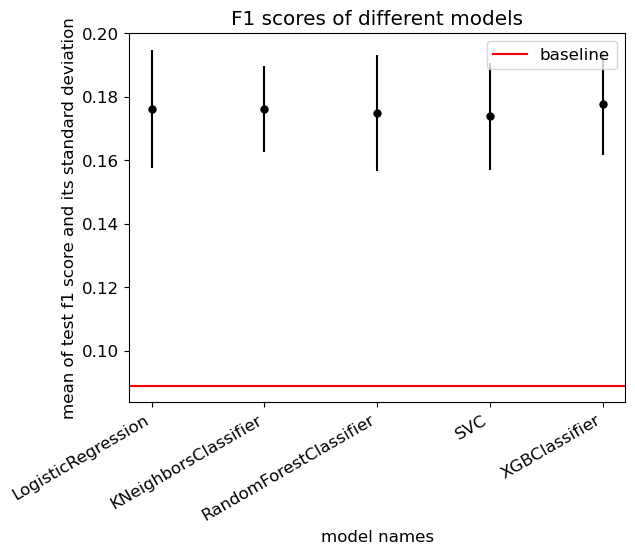
\includegraphics[width=0.65\linewidth]{models_accuracy.png}
\caption{F1 scores and the associated standard deviation for all models}
\end{figure}
\\
The best-performing model is the XGBoost classifier. Its average F1 score across different random states is 0.178, which is 5.49 standard deviations above the baseline. Out of the ten different random states, there are some variations among the best-performing hyperparameter combinations found through K-fold validation. However, the most commonly recurring combination is learning\_rate = 0.03, max\_depth = 10, and n\_estimators = 100. 
\subsection{Feature Importance}
\subsubsection{Global Feature Importance}
To illustrate the differences and similarities in global feature importance of different models, sklearn’s permutation\_importance is applied to the first and second best-performing models, i.e. XGBoost classifier and logistic regression. For the XGBoost model, the top five most important features are sensation-seeking (SS), age, openness to experience (Oscore), education, and conscientiousness (Cscore) (Fig. 7). On the other hand, the logistic regression model included openness to experience (Oscore), age, education, conscientiousness (Cscore), and impulsiveness as the five most globally important features (Fig. 8). From this it is safe to conclude that there is significant overlap between what features these two models consider to be important globally. And overall for these models, the psychological traits, age, and education have more predictive power over other features. 
\begin{figure}[!h]
\centering
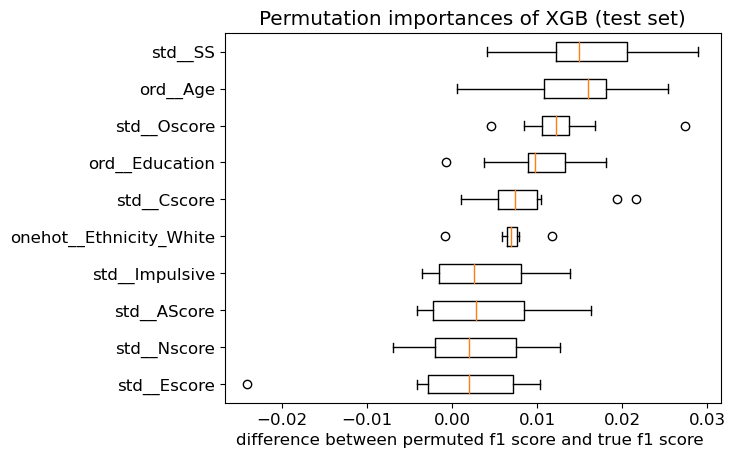
\includegraphics[width=0.75\linewidth]{XGB_permutation.png}
\caption{Important features of XGBoost classifier from permutation importance}
\end{figure}
\begin{figure}[!h]
\centering
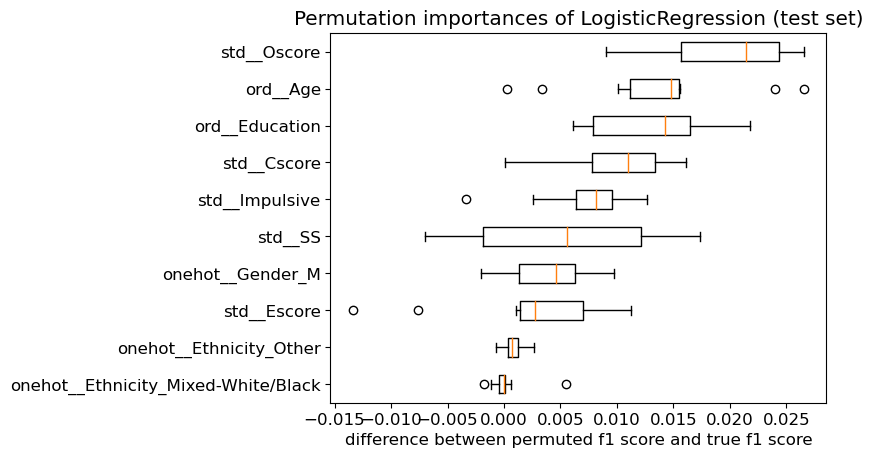
\includegraphics[width=0.85\linewidth]{LogisticRegression_permutation.png}
\caption{Important features of logistic regression from permutation importance}
\end{figure}
\\
To further illustrate the global feature importance of the model with the highest predictive power, the shap.TreeExplainer package is used to calculate the SHAP values of the XGBoost classifier, and a summary plot is created (Fig. 9).  With this measure of global importance, the top five features of interest are sensation-seeking (SS), age, openness to experience (Oscore), conscientiousness (Cscore), and agreeableness (A). These coincide with many of the important features measured with feature perturbation, further confirming their contribution to the model. 

\begin{figure}[!h]
\centering
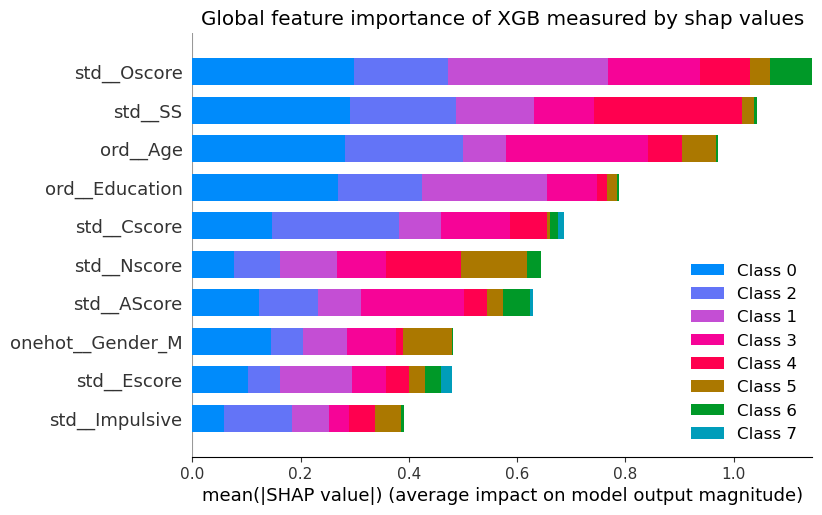
\includegraphics[width=0.85\linewidth]{XGB_shap.png}
\caption{Important features of XGBoost classifier from SHAP}
\end{figure}

\subsubsection{Local Feature Importance}
The above-mentioned SHAP values are also used to interpret the XGBoost model's prediction on single data points. Two examples of local feature importances plotted using SHAP force\_plot are shown in Figures 10 and 11. For both of these plots, the class of interest is set to 0. The first data point has a true class label of 3 and a SHAP value smaller than the base value for class 0. Attributes that are influencing this prediction are younger age, higher sensation-seeking (SS) score, less education, and higher openness to experience (Oscore). Whereas the second data point has a true class label of 0 and a SHAP value greater than the base value for class 0. Factors positively contributing to its higher-than-average SHAP value include lower sensation-seeking (SS) score, older age, greater amount of education, and higher conscientiousness (Cscore) score. 
\begin{figure}[!h]
\centering
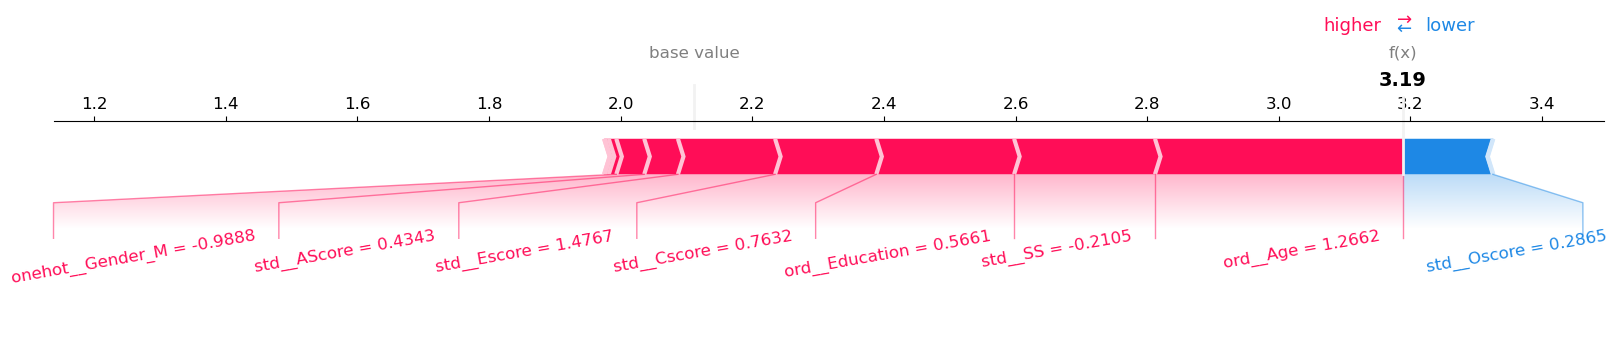
\includegraphics[width=1\linewidth]{shap_1.png}
\caption{Important features of XGBoost classifier's prediction on one data point}
\end{figure}

\begin{figure}[!h]
\centering
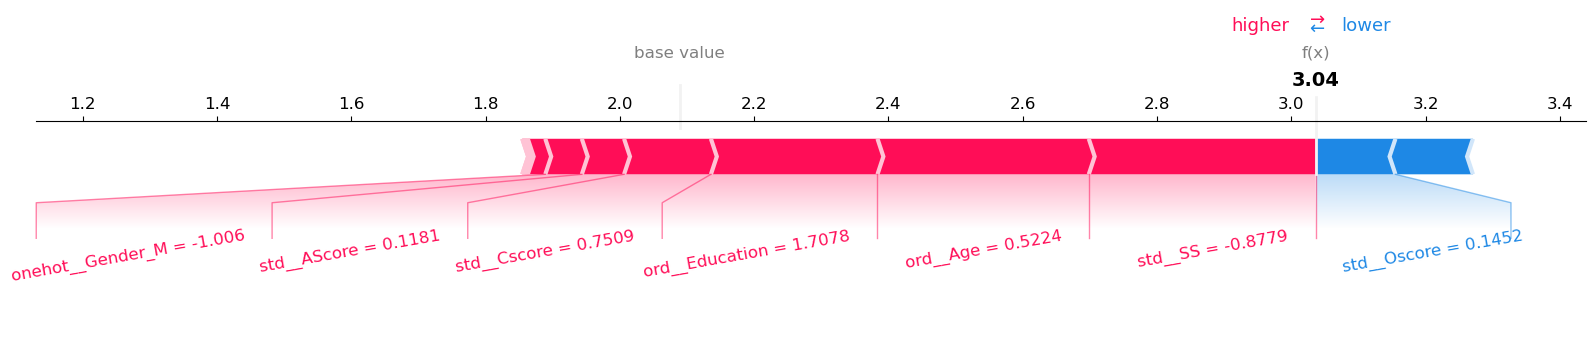
\includegraphics[width=1\linewidth]{shap_2.png}
\caption{Important features of XGBoost classifier's prediction on another data point}
\end{figure}

\subsubsection{Interpretations}
These globally and locally important features agree for the most part, and remain consistent across different measurement strategies, e.g. feature perturbation and SHAP.  The importance of different psychological traits and demographics as well as the direction in which each attribute influences the prediction aligns with the expectation of this study. For example, as shown in Figure 5 of the EDA section, the Sensation Seeking (SS) score is positively correlated to drug use. This correlation reoccurred as the most important feature for XGBoost in both permutation importance and global SHAP, as well as in the local SHAP force plots. However, during EDA, the use of legal substances, especially tobacco, was strongly linearly correlated with the target variable, but these features are unexpectedly among the least important features in the final models. Broadly speaking, in the context of the problem, the model interpretations are also in line with the general stigma around people who tend to become drug abusers. 

\section{Outlook}
Given the time limit of this study, there remains great scope for improvement. Preferably, different models could be applied to the dataset, and for the already trained models, further hyperparameter fine-tuning could be done.\\
\\
The greatest limitation of the models is that, even though the F1 score with macro averaging is used to minimize false negative rates on smaller label classes, the models do not perform ideally on those classes as shown in the confusion matrix of the XGBoost model (Fig. 12). This is probably due to the severely unbalanced distribution of the dataset. An alternative, binary classification model that distinguishes non-drug users (class 0) and drug users (class 1 through 7) might be more suitable. 
\begin{figure}[!h]
\centering
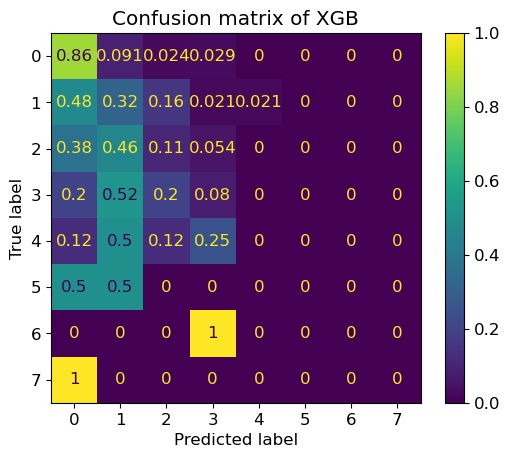
\includegraphics[width=0.7\linewidth]{XGB_confusion_matrix.png}
\caption{Confusion matrix showing the XGB model have lower predictive power for higher label classes}
\end{figure}

\pagebreak
	% bibliography style is set to SIAM here. you can experiment with other styles
	\bibliographystyle{siam}
	
	% this line includes all references cited in the document. 
	\bibliography{references.bib}
	
\end{document}
